\section{Variable Type Generation Model}
\label{sec:type-gen}

\begin{figure*}[ht]
	\begin{center}
	  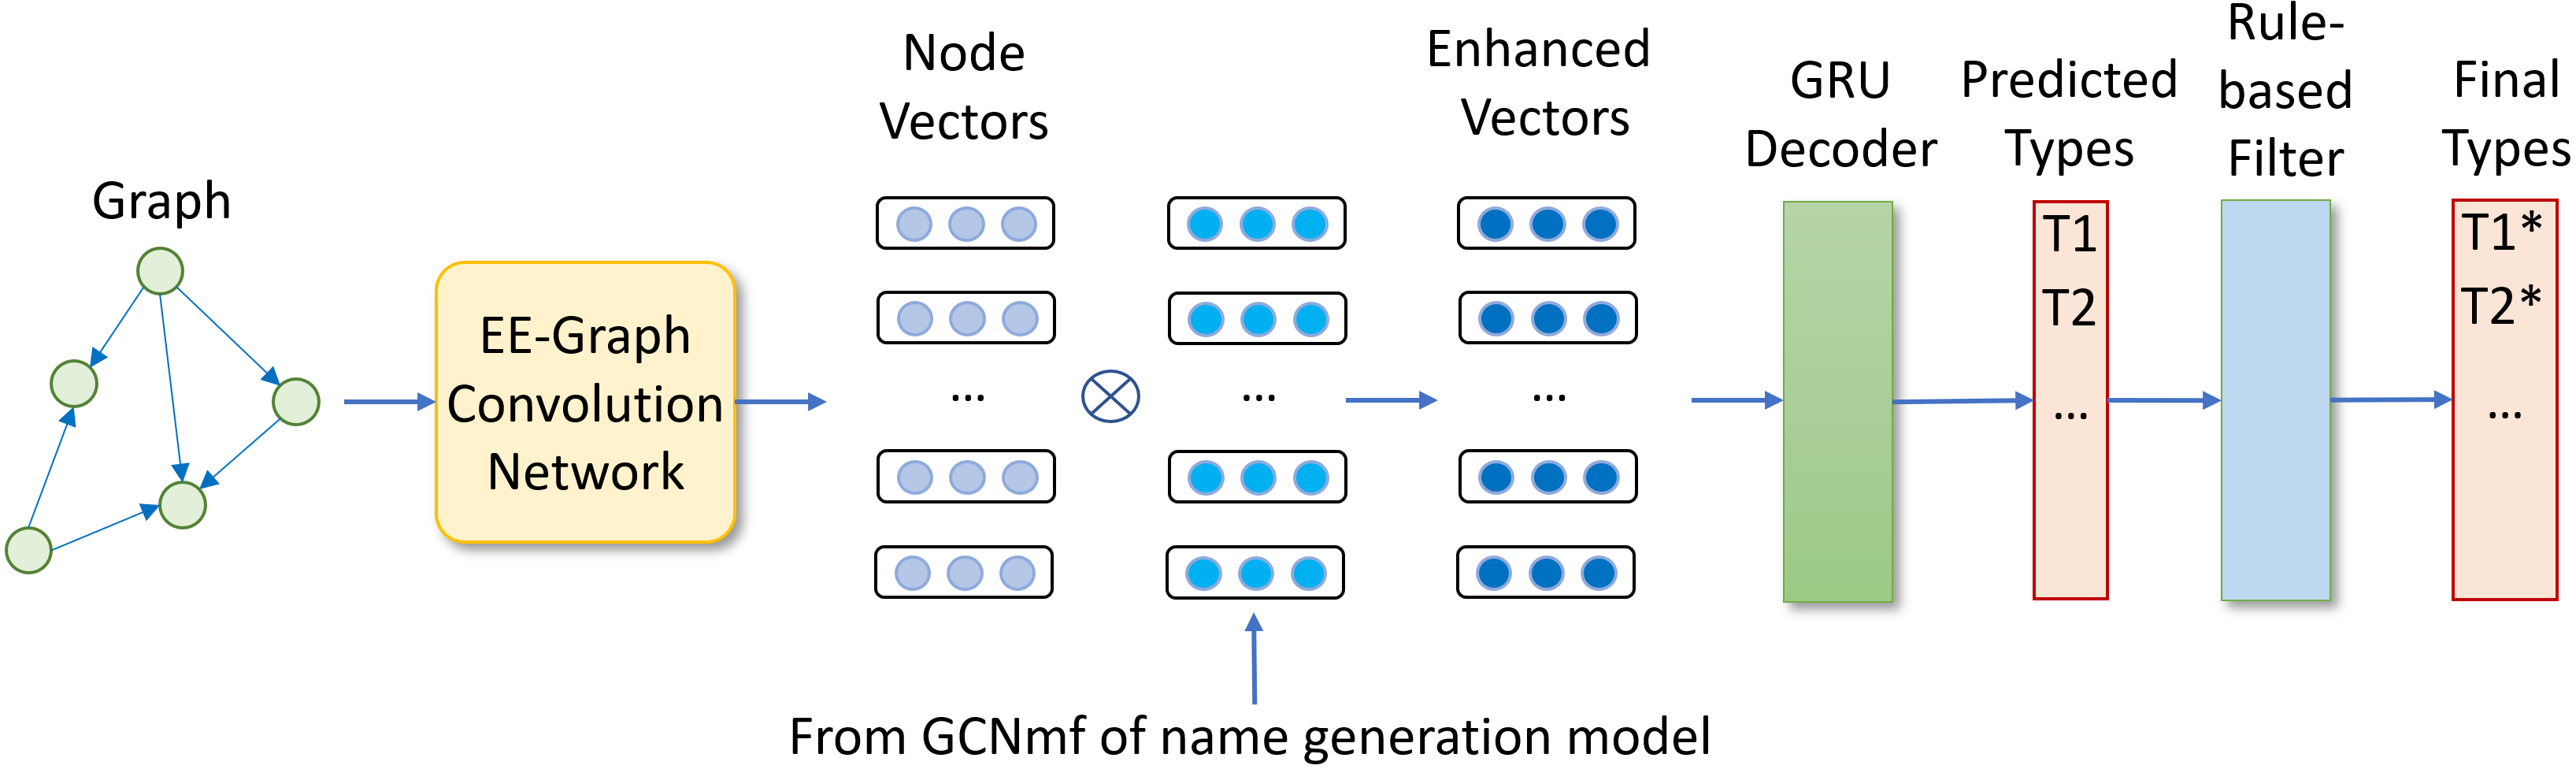
\includegraphics[width=5in]{figures/type-gen-model}
          \vspace{-6pt}
		\caption{The Variable Type Generation Model (VTG)}
		\label{fig:type-gen}
	\end{center}
\end{figure*}

This section presents the Variable Type Generation Model (VTG).

Variable Type Generation:

1> Graph edge represent different relations (This may change depends on the graph we finally want to use). Each node is a variable, method call, or a field of an object. We use the name of the variable (minified), method call, or the field as the node feature and use GloVe to learn the representation vector.

2> We use EGCN that accepts graphs with both node features and edges features as input. Here the edge feature is the edge type. 

3> The output of EGCN is the generated representation vector $V_r$ for each node. 

4> We combined the representation vector we get from EGCN with the generated from the next step $V'_r$ (variable name generation) by using the cross-product and get the final generated representation vector for type prediction ($V_f$)

5> We use a GRU (RNN) as decoder accepts the $V_f$ as input and generates the type for the variables as output.

6> When generating the type, we use some basic rule from parser to reduce the possible candidates.
